\documentclass{article}[]
\usepackage{epsfig}
\usepackage{psfig}
\usepackage{graphicx}
\usepackage{url}
\usepackage{listings}

\begin{document}

\title{{\bf Hybrid Particle Swarm Optimization with Simulated Annealing for the Travelling Salesman Problem }\\ }

\author{Student name:\\\vspace{0.5cm}EvanO'Keeffe\\ 
 Student number:\\ \vspace{0.5cm} 10324289}

\date{November 25 2013}
\maketitle
\begin{abstract}
Particle Swarm Optimization (PSO), is one of many intelligent computation algorithms which is based off the simulation of bird swarms.PSO is well known to solve continuous problems , but with modifying it with other heuristics it can be used to solve discrete problems such as the classical test model : the Travelling Salesman Problem (TSP).In this paper the PSO algorithm will have another set of heuristics working with it, mainly the Simulated Annealing heuristic .The name and inspiration come from annealing in metallurgy, a technique involving heating and controlled cooling of a material to increase the size of its crystals and reduce their defects . This works as a slow decrease in the probability of accepting worse solutions as it explores the solution space. As the time required to find a solution reaches its end , a temperature value is decreased to allow "worse" moves to be made . This allows the overall algorithm to search a larger space and as such, it will have a higher probability of finding a better route which is represented by the scores in pbest and gbest in PSO. We hope to see by hybridizing PSO with Simulated Annealing can a better result be obtained and with less variance than if a regular PSO algorithm were to be used with the Travelling Salesman problem.
\end{abstract}

\section{Introduction}
\subsection{Travelling Salesman Problem}
Travelling salesman problem is a well known NP-complete problem as a benchmark for new algorithms. The problem is describe as the following: Suppose that there is a salesman who wants to visit a number of cities (say n cities), his objective is to find the shortest route through which he can visit all cities once and only once and finally return to the starting city.The computational cost of exhaustive permutations of Travelling Salesman is O(n!). At the time of this paper a number of studies have been conducted using the TSP benchmark in Ai such as neural networks\cite{Gee1995} .Areas of natural computing have been shown to work very well such as genetic algorithms\cite{Ray2004},simulated annealing\cite{Song2003}, ant colony optimization\cite{Dorigo1996}, river formation dynamics\cite{Afaq2011} etc...
\subsection{Particle Swarm Optimization}
Particle Swarm Optimization is a evolutionary algorithm that was proposed by Eberhart and Kennedy in 1995\cite{Kennedy1995}. It is based off the simplified model of the social system of flying bird swarms. Each bird(or particle) in the swarm will attempt to get to the best point in the swarm. It will search the whole space by using its previous best position (pBest) and the best global position in the swarm (gBest). PSO is very successful in that it is easy to implement and has a high performance in continuous search spaces. It has however been found that when applying PSO to discrete areas such as the Travelling Salesman that it does not however prove to work as efficiently as other algorithms.

\subsection{Simulated Annealing}
Simulated annealing (SA) is a probabilistic meta-heuristic for the global optimization problem of locating a good approximation to the global search space optimum of a given function in large search spaces.It was first described by Scott Kirkpatrick, C. Daniel Gelatt and Mario P. Vecchi in 1983,\cite{Kirkpatrick1983} and by Vlado Černý in 1985\cite{JournalofOptimizationTheoryandApplications1985}. The method is an adaptation of the Metropolis-Hastings algorithm, a Monte Carlo method to generate sample states of a thermodynamic system, invented by M.N. Rosenbluth and published in a paper by N. Metropolis et al. in 1953.\cite{Metropolis1953}

In this paper we hope to use the properties of simulated annealing with particle swarm optimization ,to allow the swarm to move into areas it would otherwise deem to not be optimal and find a better scoring route than the standalone PSO algorithm. 

\newpage
\section{Algorithms}
\subsection{Basic Particle Swarm Optimization Algorithm}
In the fundamental PSO model, a particle swarm stands for a flock of birds and searches for the solution in D-dimensional real space.Each particle has it's own position vector (a valid solution) and velocity vector (decides the particle's next next action), which are both D-dimension. The fitness of each particle should be determined by a unique function to estimate the quality of the particle.
 
The system is initialized with a population of random solutions and searches for optima by updating potential solution over each generation. In PSO, the potential solutions (or particles), move through the problem space by following the current better performing particle. The solution updating can be represented by the concept of velocity. By definition, a velocity is a vector or, more precisely, an operator, which, applied to a position (solution), will give another position (solution). It is in fact a displacement, called velocity because the time increment of the iteration is always implicitly regarded as equal to 1 .\\Velocity of each particle can be modified by the following equation:
\begin{equation}
\label{particleUpdate}
v_i,_d \leftarrow \omega v_i,_d + \phi_p  r_p (p_i,d-x_i,_d) + \phi_g  r_g (g_d - x_i,_d)
\end{equation}
\cite{Russell2003}
This can be represented in the following pseduo code below
\newpage

\begin{figure}[bottom] 
\centering
\begin{lstlisting}
Randomly initialize the whole swarm
for(i = 0; i < size of swarm ; i++){
	Evaluate fitness(x_i)
}
while(optimum state has not been found or max iterations reached){
	for(i=0; i < size of swarm; i++){
		if(fitness(x_i) > fitness(pbest_i){
			pbest_i = x_i;
		}
		if(fitness(x_i) > fitness(gbest)){
			gbest = x_i;
		}
		update(x_i,v_i);
		Evaluating fitness(x_i)
	}
}
\end{lstlisting}
\caption{PSO Pseudo Code}%
\label{PSO-Code}%
\end{figure}

\subsection{Simulated Annealing Algorithm}
In statistical mechanics , a physical process called annealing is used to preform a relaxation in the systems state with minimum free energy. It consists in using a control parameter in the optimization, which plays the rule of temperature. The temperature of the system to be optimized must have the same effect as the temperature of the physical system: it must condition the number of accessible states and lead to the optimal state.If the temperature is lowered gradually in a controlled manner it should lead to the optimal state and towards a local minimum if the temperature is lowered abruptly.\\

$\Delta$E$\le$0 (i.e the newest state is better than the current state) the modification will be accepted.When it is $\Delta$E$>$0 if the probability exp(- $\Delta$E/T) is greater than a random number drawn uniformly between 0 and 1, the modification making the state worse will also be accepted(Metropolis rule\cite{Metropolis1953}).Essentially this allows the algorithm to reach other parts of the search space that at the time would not have been searched due to low fitness in the area. The pseudo code in figure \ref{SA-Code} shows how this is implemented
\cite{Russell2003}

\newpage
\begin{figure}[bottom]
\centering
\begin{lstlisting}
s = s0
e = E(s)
sbest = s
ebest = e
k = 0
while (k < kmax AND e > emax){
	T = temperature(k / kmax)
	snew = neighbour(s)
	enew = E(snew)
	if(P(e,enew,T) > random()){
		s = snew
		e = enew
	}
	if(enew < ebest){
		sbest = snew
		ebest = enew
	}
	k = k + 1
}
\end{lstlisting}
\caption{Simulated Annealing Pseudo Code}%
\label{SA-Code}%
\end{figure}
\newpage
\subsection{Particle Swarm Optimization with Simulated Annealing Algorithm}
The algorithm functions much like the standard PSO algorithm.
\begin{itemize}
\item Firstly we generate the number of particles with random initial states
\item Next we preform the updating functions on each particle
\item If the local maximum has not been found yet , repeat previous statement
\item Select the particle with the best state
\item Start the Simulated Annealing with the selection result
\item Generate the Initial temperature ( float("inf") was used )
\item modify the state and accept according to the metropolis rule\cite{Metropolis1953}
\item if the state evaluates to zero then the final state i.e the optima searched for has been reached , if not then repeat the selection of the new best state and repeat procedure
\item Decrease the temperature in a controlled fashion (we used T * 0.99 )
\item end of algorithm
\end{itemize}
\label{psosaAlg}


\newpage
\section{Procedure}
The experiment was conducted using two separate python script files. One with only a PSO algorithm in it, the other
with the hybrid PSO-SA algorithm.The scripts were run on an Intel i3 quad-core at 1.90GHz with 4GB or ram using the input parameters in table \ref{table:params}. Each run of the test is saved into a spreadsheet that can then be read by the user.
\begin{table} 
\caption{Input Parameters Used} % title of Table 
\centering      % used for centering table 
\begin{tabular}{l|c}  % centered columns
\hline                      %inserts double horizontal lines 
{\bf Parameter}&{\bf Value}\\
%heading 
\hline                    % inserts single horizontal line 
Total Iterations & 200\\
Error Margin & approximately 7\% \\
Number of Particles & 10\\
Maximum Velocity & 4\\
Epoch  & 10000\\
Number of Cities & 100\\
\hline     %inserts single line 
\end{tabular} 
\label{table:params} 
 \end{table} 

\section{Results}
The results received from the above procedure (item \ref{psosaAlg}) shown in table \ref{table:results}, show that the PSO-SA algorithm was able to out preform the standard PSO algorithm. Going through the data we can see that while the best score received by PSO-SA was only slightly greater than the PSO , we can see the standard deviation of the PSO-SA algorithm is far less than its PSO counterpart. The Mean Average Score in PSO-SA also showed that while its average was nearly similar to PSO , its deviation from the average was nearly a factor of two smaller. This means that the PSO-SA was able to consistently make better selections on new particle states than PSO.

\begin{table} [b]
\caption{Results Table} % title of Table 
\centering      % used for centering table 
\begin{tabular}{l|c|c}  % centered columns
\hline                      %inserts double horizontal lines 
{\bf }&{\bf PSO}&{\bf PSO-SA}\\
%heading 
\hline                    % inserts single horizontal line 
Average Best Score & 4043.987 & 4130.891\\
Best Score Standard Deviation &  135.105 & 78.852\\
Mean Average Best Score & 4119.442 & 4181.567\\
Mean Average Best Score Standard Deviation &  182.0345 & 96.649\\
Average Time(seconds) & 109.328 & 108.8475\\
\hline     %inserts single line 
\end{tabular} 
\label{table:results} 
 \end{table} 

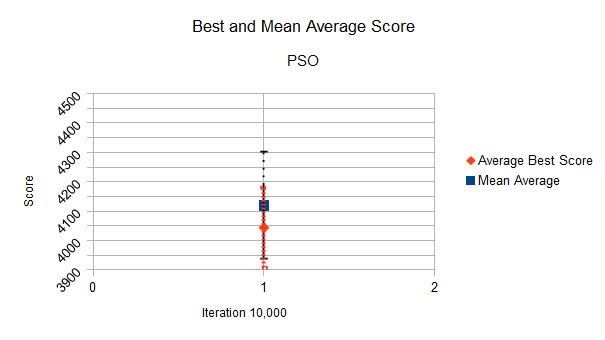
\includegraphics[scale=0.8]{bestAndAverageScore-PSO.png}
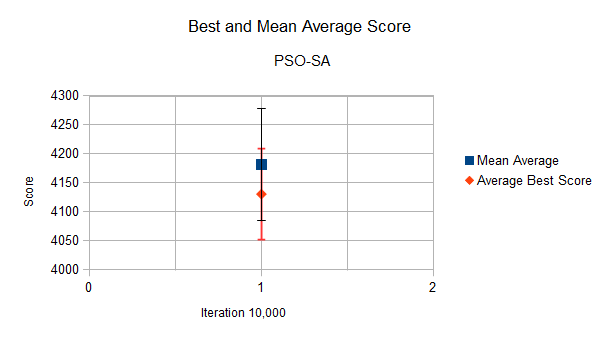
\includegraphics[scale=0.8]{bestAndAverageScore-PSOSA.png}
The results show in both the above plots show that we received a more stable standard deviation with our PSO-SA algorithm. The average score that was taken by iteration 10,000.

\section{Conclusions}
There is conclusive evidence that by mixing the Simulated Annealing heuritic with PSO ,we obtained rewarding results in both the best score obtained at the end , the best score that was found on average and also the better standard deviation of the scores over the number of the iterations with the hybrid algorithm.
All the code is accessible at https://github.com/eokeeffe/Natural-Computing with a readme.txt that explains how to run the programs

\section{Future Work}
Firstly we would like to note that it would have also been interesting to see the pBest and gBest during the runtime of the algorithms to see which of the algorithms arrived at a better solution first. This is something we could do in the next iteration of tests using these parameters.
This experiment shows that it is possible to mix meta-heuristics with PSO to enhance the algorithm. It would be interesting to see what the effect of mixing other natural computing heuristics like dynamic river formation with SA and PSO would enhance the results or else see if it could theoretically work in other classical model tests.  

%ACKNOWLEDGEMENTS are optional
\section{Acknowledgements}
We would like to firstly thank Dr. Michael O'Neill and Dr. Miguel Nicolau of the UCD NCRA for their guidance and support during the write up of this work.\\
We would like to also thank John McCullock @
\url{http://mnemstudio.org/} for the starting python code for the travelling salesman problem PSO solution.\\
Dr.Saffarzadeh for the paper on simulated annealing for NQueen problem which helped in my understanding of hybridizing meta-heuristics \cite{Saffarzadeh2010}
and Dr.Wen-Liang Zhong for his research on multistage PSO which helped in my understanding of how to integrate SA with PSO\cite{Zhong2007}

\bibliographystyle{abbrv}
\bibliography{backup2}


\end{document}